\lettrine[lines=3]{P}{}rocedurally generating 3D models of plant-life is a challenging task, largely due to the complex branching structures and variation between different types of plant species. Up until recently, all assets within 3D graphics applications either had to be sculpted using 3D modeling software or scanned using photogrammetry, laser triangulation or some form of contact-based 3D scanning. These methods are still used today but tend to be very time consuming and extremely costly. With the increase in computational power over the last few decades more emphasis has been placed on the use of procedural generation. Which can be used to create complex structures such as terrain, architecture, sound and 3D models with far greater speed than previous techniques, and often much better realism than would be possible with artists. Plant-life stands as a challenge due to the thousands of species, each with their unique structure and features. It is difficult to define a system that can represent them all in a way that is simple, understandable and accurate. The Lindenmayer System (L-system) stands as a solution to this problem, it was originally developed by Aristed Lindenmayer as a method of representing the development of multicellular organisms \cite{lindenmayer1968mathematical}. This has since gained popularity in the area of procedural generation and has been adapted to represent different types of structures. L-systems have been adapted to represent plant-life, such as trees, flowers, algae, and grasses. Whilst still applying to non-organic structures such as music, artificial neural networks, and tiling patterns \cite{Prusinkiewicz1989}.

\section{Motivations}

The L-system, in its most basic form, is a formal grammar that contains a set of symbols or letters that belong to an \textit{alphabet}. A starting string or \textit{axiom} is created using the alphabet, as well as a set of production rules. The production rules are applied to each symbol within the axiom string, and each rule dictates whether or not the symbol can be rewritten and what they will be rewritten with. In essence, an L-system uses the set of production rules to generate a resulting string of symbols which follow those production rules. What the resulting strings' is ultimately going to represent depends on how it is interpreted. In this case, the string of symbols can be interpreted to generate a model of a plant. This thesis develops upon the L-system concepts described by Przemyslaw Prusinkiewicz and Aristid Lindenmayer to procedurally generate structures of plant-life in real-time. The L-system grammar allows the construction of a plant to be described in a human-readable, formal grammar. The grammar can be used to specify variation in shape, size, and branching structure within a particular species. Furthermore, this thesis will also investigate the use of a parameterised L-systems to provide physical properties using string rewriting. Which in turn will enable the animation and physical behavior of the plant that it generates, thus making it possible to simulate external forces such as gravity and wind.\\

This chapter will provide an overview for how to improve the procedural generation of plant-life in 3D applications and the motivations doing so. It will then introduce the concepts of procedural generation, rewriting systems, and formal grammars. This chapter will briefly describe how to apply procedural generation to the development of plant-life, and will provide sufficient background as to the use of formal grammars as a means of describing complex L-system languages. Finally, there will be an outline as to the structure of this thesis.

\section{Introduction to Procedural Generation}

Procedural generation is used in many different areas and applications in computer graphics, particularly when generating naturally occurring structures such as plants or terrain. An effective procedural generator is capable of taking input in the form of a relatively simple description of what it should be generating; its job is then to computationally create the structure in a way that is accurate to the description given. Currently, there are three main methods for procedurally generating models of plant-life; these are genetic algorithms \cite{haubenwallner2017shapegenetics}, space colonisation algorithms\cite{juuso2017procedural}, and L-systems. The genetic algorithm and space colonisation algorithms are similar in that they require the overall shape of the plant to be described by simple 3D shapes; the algorithm then creates a branching structure that matches these shapes. The limitation of these methods is that the 3D description is not very specific, and although it can get good results for trees, it may not be able to generate different types of plant-life, such as flowers. The L-system, on the other hand, relies on a method of string rewriting, whereby the rewriting is based on a set of production rules to generate a string of symbols that obey those rules. A separate system can later interpret this string to create the model. The L-system procedural generation, therefore, has two different systems within it, one of string rewriting and one of interpretation of the generated string. This makes it quite easy for the same L-system to generate very different results based upon the interpretation.\\

Plant-life can have very complex and seemingly random structures; however, with closer observation, trees of a similar species have distinct traits and features. For instance, a palm tree has long straight trunks with large compound leaves exclusively near the top, branching in all different directions. Comparatively, a pine tree has a long straight trunk with many branches coming off in different directions perpendicular to the ground, from its base to the top of the trunk. These are two very different species of trees; the palm belongs to the Arecaceae family, whereby the pine belongs to the Pinaceae family. They look different; however, they share very similar properties, such as their long straight trunks. The challenge behind the procedural generation of plant-life is providing a human-readable grammar that describes in sufficient detail, how to generate a 3D model. Whilst allowing for randomness and variety within the generation process, such that variations of a particular species can be created without repetition. The grammar for procedural generation should also be relatively straightforward and intuitive, and must accurately represent what it is going to generate. Furthermore, the description must not be limited to only known species of trees, as some graphics applications may require something other-worldly.

\section{Introduction to Rewriting Systems}

Rewriting systems are the fundamental concept behind L-systems. In their most basic form, rewrite systems are a set of symbols or states, and a set of relations or production rules that dictate how to transform from one state to the other \cite{prusinkiewicz2012algorithmic}. These production rules can be used to generate complex structures by successively replacing parts of a simple initial object with more complex parts. Rewrite systems can be non-deterministic, meaning that there could be a transition that depends on a condition being met or on neighbouring states. The rewriting concept means that any next state can rely upon some conditions necessary for transformation. If the condition evaluates true, the state is rewritten; otherwise, it remains the same and is checked in the next rewriting stage. A graphical representation of an object defined in rewriting rules can be seen below in figure \ref{snowflake curve} below, called the snowflake curve proposed by Von Koch \cite{koch1906methode}.

\begin{figure}[htbp]
	{\centering
		\setlength{\fboxrule}{1pt}
		\vspace{7px}
		\fbox{
			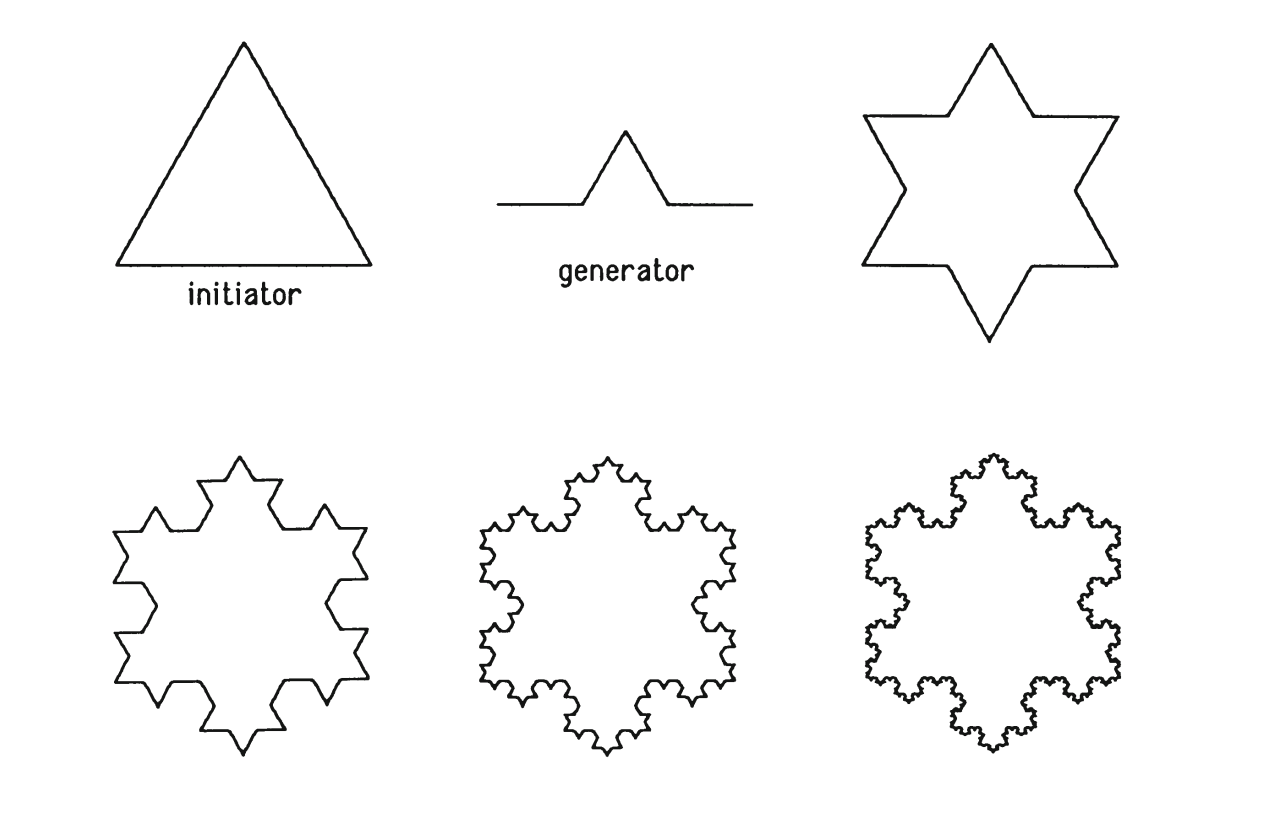
\includegraphics[scale=0.3]{Diagrams/snowflakeCurve.png}
		}
		\caption{Construction of the snowflake curve\cite{prusinkiewicz2013lindenmayer}.} \label{snowflake curve}
	}
\end{figure}
\FloatBarrier

\noindent
The snowflake curve starts with two parts, the initiator and the generator. The initiator is the initial set of edges forming a certain shape, whereas the generator is a set of edges that can be used to replace each edge of the initiator to form a new shape. That new shape then becomes the initiator for the next generation, where the generator again replaces each edge. The result is a complex shape similar to that of a snowflake. The initiator, generator concept, is a graphical representation of how rewriting systems operate; rather than the initiator and generator being a set of edges, a set of symbols or strings instead represents them.

\section{Introduction to Formal Grammars}

In the context of computer science, a grammar is defined as a set of rules governing which strings are valid or allowable in a language or text. They consist of syntax, morphology, and semantics. Formal languages have been defined in the form of grammars to suit particular problem domains. It is natural for humans to communicate a problem or solution in the form of language; it is intuitive to use a language to describe the desired outcome when dealing with the procedural generation of plant-life. In the past, formal grammars have been used extensively in computer science in the form of programming languages in which humans can provide a computer with a set of instructions to carry out to gain an expected result. The challenge is to procedural generation of plant-life by creating a  grammar in the form of a rewriting system. A rewriting system such as the L-system operates in a way that is consistent with a context-free class of Chomsky grammar \cite{chomsky1956three}, similar to that of the programming language ALGOL-60 introduced by Backus and Naur in  1960\cite{backus1960report}. In figure \ref{chomsky grammars} below, two types of L-system grammars overlap the classes of Chomsky grammars, the OL-system, and the 1L-system. The details of these two systems will be discussed in detail chapter \ref{l-system chapter}, but in summary, 0L-systems are grammars that can represent a context-sensitive Chomsky grammar but generally tend to be context-free, the main difference between the 0L-system and the 1L-system is that 1L-systems can be recursively enumerable. Furthermore, a 1L-system can represent any 0L-system, and 1L-system languages tend to be more complex and verbose when compared to 0L-systems. These two different types of L-systems each have trade-offs, 1L-systems are more powerful and complex, and 0L-systems are less powerful but make for a simpler language. 

\begin{figure}[htbp]
	{\centering
		\setlength{\fboxrule}{1pt}
		\vspace{7px}
		\fbox{
			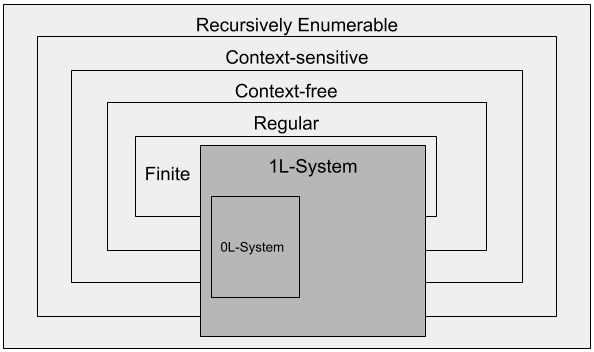
\includegraphics[scale=0.7]{Diagrams/ChomskyGrammar.png}
		}
		\caption{Diagram of the Chomsky hierarchy grammars with relation to the 0L and 1L systems generated by L-systems.} \label{chomsky grammars}
	}
\end{figure}
\FloatBarrier

\newpage

\section{Structure of Thesis}

This thesis begins by delving into the underlying concepts of L-systems. Firstly by defining the simplest type of L-system named the DOL-system. Then to provide details about how DOL-systems are interpreted to produce graphical representations. The L-system chapter provides a formal definition for more complex types of L-systems known as parametric L-systems. In conjunction with this, the L-system chapter talks about significant features and improvements that aid the procedural generation of realistic plant life. These include branching, conditionals, randomness, and stochastic rules.

Chapter \ref{rewriter chapter} focuses on the implementation of the L-system rewriter. This includes the definition of the parametric L-system grammar and syntax that will be used to develop the rewriting system software. It also describes the process of string rewriting, and computationally understanding the L-system grammar using lexical analysis and parsing as well as the string rewriting algorithm and its connection to the string interpretation process.

Chapter \ref{maths chapter} covers specific mathematical concepts necessary for working with 3D graphics. The chapter includes vectors, matrix transformations, and quaternions. The mathematics chapter is there to provide a brief overview of the concepts often used when rendering 3D graphics or simulating physical systems.  

Chapter \ref{interpreter implementation} discusses the three major stages of L-system string interpretation for the procedural generation of 3D plant-life. These consist of the turtle graphics interpreter, model generator, and renderer. The turtle graphics interpreter explains the process of creating the trees' skeletal structure. The model generator discusses how to generate the vertex data for the 3D models of the plants using a skeletal structure, which can create a realistic-looking plant. Finally, the renderer covers the specifics of rendering models on the screen in the OpenGL framework.

The physics simulator chapter focuses on a straightforward method to simulate wind and gravitational forces on 3D generated plants. This chapter includes details of Hook's Law and the equations of motion that are implemented within the simulator.

The results chapter \ref{results chapter} highlights a number of results produced by the L-system and discusses how the L-system can be used to manipulate the generated plant models as well as their physical behaviour when simulated. 